\begin{figure}
  \centering
  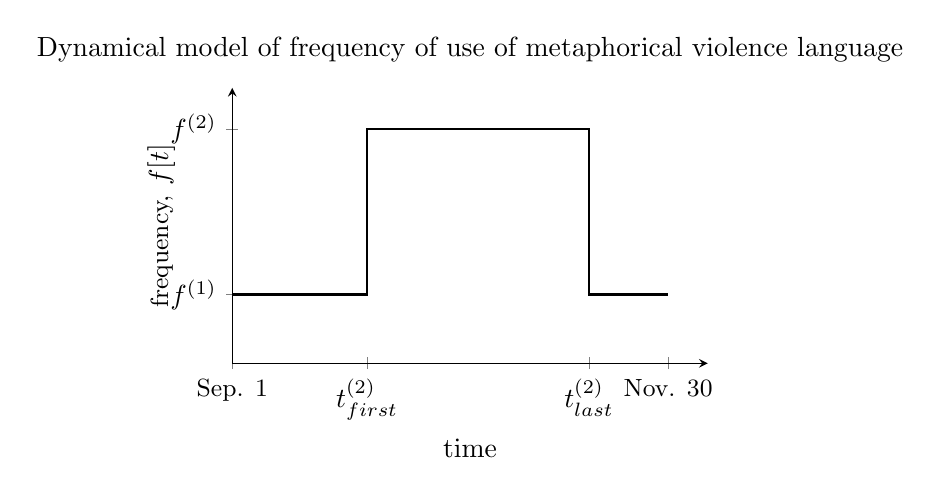
\begin{tikzpicture}
    \begin{axis}[%
      ,xlabel=time
      ,ylabel={{\small frequency,} $f[t]$}
      ,axis x line = bottom,axis y line = left
      ,xmax=3.25
      ,xtick={0.25, 1.1, 2.5, 3}
      ,xticklabels={{\small Sep. 1}, $t_{first}^{(2)}$, $t_{last}^{(2)}$, {\small Nov. 30}}
      ,ytick={.5, 1.7}
      ,y label style={at={(axis description cs:-0.10,.5)}}
      ,yticklabels={$f^{(1)}$, $f^{(2)}$}
      ,ymax=2.0 % or enlarge y limits=upper
      ,ymin=0.0
      ,title={Dynamical model of frequency of use of metaphorical violence language}
      ,width=3.0in
      ,height=2.0in
      ]
      \addplot+[const plot, no marks, thick, black] coordinates {(0.25,.5) (1.1,1.7) (2.5,.5) (3, .5)};
    \end{axis}
  \end{tikzpicture}
  \caption{Illustration of the dynamical model of Equation 1. 
    We determine $t^{(2)}_{first}$, $t^{(2)}_{last}$, $f^{(1)}$, and $f^{(2)}$
    for six time series (two shows on three networks in 2012 and 2016) 
    through Bayesian inference. 
    }
  \label{fig:model-illustration}
\end{figure}
